\documentclass[11pt,openany]{book}
% #1-Asignatura
% #2-Curso
% #3-Nombre
% #4-Link
% #5-Foto

\newcommand{\portada}[5]{
    \begin{titlepage}
        \begin{center}
            \vspace*{0.5cm}
            
            % Titulo con #1 lo mas grande posible
            {\Huge \textbf{#1}}

            
            \vspace{0.5cm}
            \LARGE
            Curso #2 
            
            \vspace{1cm}
            
            \Huge{\textbf{Grupo Viterbi}}

            \vspace{1cm}
            
\includegraphics[width=0.6\textwidth]{assets/Img/UGR-Logo.png}
            
            \vspace{0.5cm}

            \huge
            PRÁCTICA 5- PROGRAMACIÓN DINÁMICA
            
            \Large
            \vspace{1cm}
            \textbf{Integrantes:}  \\ 
             % Array con los nombres de los integrantes y el correo
             \begin{center}
                \begin{tabular}{c c }
                    \textbf{Miguel Ángel De la Vega Rodríguez} & miguevrod@correo.ugr.es \\
                    \textbf{Alberto De la Vera Sánchez} & joaquinrojo724@correo.ugr.es \\
                    \textbf{Joaquín Avilés De la Fuente} & adelaveras01@correo.ugr.es \\
                    \textbf{Manuel Gomez Rubio} & e.manuelgmez@go.ugr.es \\
                    \textbf{Pablo Linari Perez} & e.pablolinari@go.ugr.es
                \end{tabular}
             \end{center}
            \vspace{0.8cm}
            
            
            \large
             \vspace{1cm}
            Facultad de Ciencias UGR\\
            Escuela Técnica Ingeniería Informática UGR\\
            Granada\\
            #2 
            
        \end{center}
    \end{titlepage}
}



\usepackage{assets/formulas}
\usepackage{float}
\hbadness=10000 % Suppress Underfull \hbox warnings

%========================================|Indice|===============================================%

\begin{document}
\portada{Algorítmica}{2023-2024}{Miguel Ángel De la Vega Rodríguez}{https://github.com/Miguevrgo/}{github.png}
\tableofcontents % Índice
\newpage %Salto de pagina tras el Indice


%======================================|Documento|==============================================%
\chapter{Autores}
\begin{itemize}
      \item \textbf{Miguel Ángel De la Vega Rodríguez:} 20\%
            \begin{itemize}
                  \item Plantilla y estructura del documento \LaTeX
                  \item Programación Viajante
                  \item Programación SumaMax (DyV)
                  \item Tests de eficiencia
            \end{itemize}
      \item \textbf{Joaquín Avilés De la Fuente:} 20\%
            \begin{itemize}
                  \item Programacion SumaMax (DyV)
                  \item Tests de eficiencia
            \end{itemize}
      \item \textbf{Alberto De la Vera Sánchez: } 20\%
            \begin{itemize}
                  \item Redacción \LaTeX
                  \item Graficas y ajustes
            \end{itemize}
      \item \textbf{Manuel Gomez Rubio} 20\%
            \begin{itemize}
                  \item Programacion SumaMax (Kadane)
                  \item Programacion Losetas
            \end{itemize}
      \item \textbf{Pablo Linari Pérez:} 20\%
            \begin{itemize}
                  \item Programacion SumaMax (Kadane)
                  \item Programacion Losetas
            \end{itemize}
\end{itemize}

\chapter{Objetivos}
En esta práctica, se pretende resolver problemas de forma eficiente aplicando la técnica de
Divide y Vencerás. Para ello, se han planteado varios problemas cuya solución es conocida
(excepto para el problema del viajante), y se han implementado algoritmos que los resuelven
mediante el método convencional y mediante la técnica de Divide y Vencerás. Posteriormente, se ha buscado
un umbral en el cual ambos tengan el mismo tiempo de ejecución, finalmente, se ha buscado el
umbral óptimo para cada problema.
\chapter{Definicion Problema}
\chapter{Algoritmo Especifico}
En este apartado, estudiaremos la eficiencia teórica, empírica e híbrida de los algoritmos especificos
de cada uno de los problemas.
\section{Problema 1: Subsecuencia de suma máxima.}
Para el primer problema, el algoritmo específico que empleamos es el algoritmo de Kadene.
\subsection{Estudio teórico}
\begin{lstlisting}
      int kadane(int *a, int size){
            int max_global = a[0];
            int max_current = a[0];

            for (int i = 1; i < size; i++) {
                  max_current = max(a[i], max_current + a[i]);
                  if (max_current > max_global) {
                        max_global = max_current;
                  }
            }
            return max_global;
      }
\end{lstlisting}
Como podemos observar la eficiencia del codigo en las líneas 6-8, tienen eficiencia O(1). Por tanto,
su tiempo de ejecución es constante y notaremos por a. Luego, el bucle for se ejecutará  $(size-1)-i+1 $
veces, es decir, $size-i$ veces. Sabiendo que el resto de líneas del código tienen eficienciaa O(1), tenemos
el siguiente resultado
\begin{equation*}
      \sum_{i=inicial}^{size-1} a
\end{equation*}
Tomaremos $size =  n$ e $inicial = 1$ para simplificar el cálculo y veamos que obtenemos ahora
\begin{equation*}
      \sum_{i=1}^{n-1} a = a \cdot \sum_{i=1}^{n-1} 1= a \cdot (n-1)
\end{equation*}
Es claro que $a \cdot (n-1) \in O(n)$ y por tanto la eficiencia teórica del algoritmo de kadane es $O(n)$.
\subsection{Estudio empírico}
\begin{center}
      \begin{figure}[H]
                  \centering
                  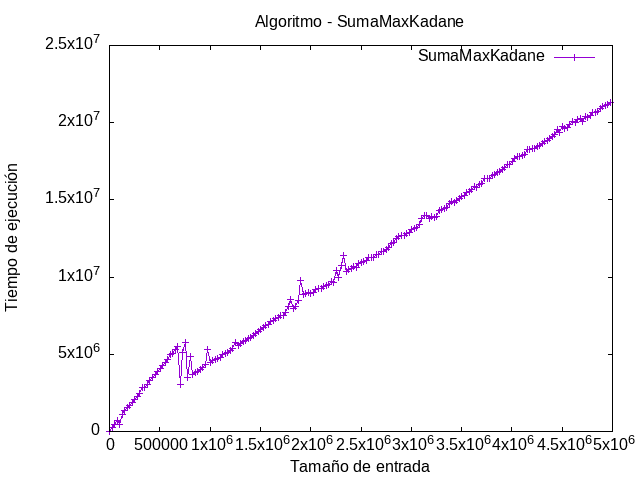
\includegraphics[width=0.7\linewidth]{assets/Img/SumaMaxKadane.png}
                  \caption{Ejecución algoritmo SumaMaxKadane}
                  \label{fig:SumaMaxKadane}
      \end{figure}
\end{center}
\subsection{Estudio híbrido}
\begin{center}
      \begin{figure}[H]
                  \centering
                  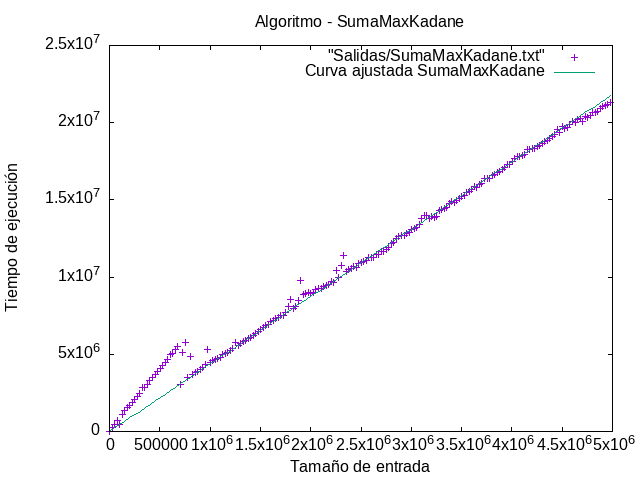
\includegraphics[width=0.7\linewidth]{assets/Img/SumaMaxKadane_hib.png}
                  \caption{Ajuste hibrido}
                  \label{fig:SumaMaxKadanehibrido}
      \end{figure}
\end{center}
Tras la interpretación de los datos empíricos en gnuplot y de la formula teorica del métoco, obtenemos que \\
las constantes ocultas son:
\begin{equation*}
      T_{Kadane}=1.64263x + 0.996451
\end{equation*}
\section{Problema 2: Enlosar un espacio }
Para el segundo problema el algoritmo específico que empleamos para resolver el problema es el siguiente : 

\begin{lstlisting}

      void resuelve2(int i,int j,int n, vector<vector<int>> & mat){
        losas++;
        for(int l = 0; l< n; l++){
            for(int k = 0; k<n; k++){
                if(mat[i+l][j+k] == 0){
                    mat[i+l][j+k] = losas;
                }
            }
        }
    
}
\end{lstlisting}
El código consiste en rellenar las posiciones de una matriz 2x2 con un valor entero en las posiciones donde el valor sea 0.
Podemos observar que hay dos bucles for anidados los cuales son $O(n)$ y el interior del bucle más profundo es $O(1)$ por tanto la eficiencia 
de este código es de $O(n^2)$

\chapter{Algoritmo Divide y Vencerás}
En este apartado, estudiaremos la eficiencia teórica, empírica e híbrida de los algoritmos divide y vencerás
de cada uno de los problemas.
\section{Problema 1: Subsecuencia de suma máxima.}
Para el primer problema, el algoritmo específico que empleamos es
\subsection{Estudio teórico}
\begin{lstlisting}
   SumaData SumaMax (int *v, int inicio, int final){
         SumaData result, d1, d2;
         if (inicio==final){
               result.max_izq = v[inicio];
               result.max_dch = v[inicio];
               result.sum = v[inicio];
               result.max_sub = v[inicio];
               return (result);
         }

         int mid = (final+inicio)/2;
         (d1)=SumaMax(v, inicio, mid);
         (d2)=SumaMax(v, mid+1, final);
            
         result.max_izq = max(d1.max_izq, d1.sum+d2.max_izq);
         result.max_dch = max(d2.max_dch, d2.sum+d1.max_dch);
         result.sum = d1.sum + d2.sum;
         int max_cross = d1.max_dch + d2.max_izq;
         result.max_sub = max(max(max_cross, d1.max_sub), d2.max_sub);
         return (result);
   }
\end{lstlisting}
Este algoritmo devuelve un tipo de dato Suma data, un struct definido por cuatro datos de tipo int. En cuanto
a la eficiencai teórica, podemos ver una llamada recursiva a la función SumaMax con vectores de tamaño $\frac{n}{2}$.
Teniendo en cuenta que el resto de líneas de código son asignaciones, comparaciones y operaciones arimtéticas, que son O(1), obtenemos
la siguiente ecuación
\begin{equation*}
      T(n)=2T(\frac{n}{2})+1
\end{equation*}
Al realizar un cambio de variable $n=2^m$(luego $m=log_2(n)$), obtenemos:
\begin{gather*}
      T(2^m)=2T(2^{m-1})+1 \\
      T(2^m)-2T(2^{m-1})=1
\end{gather*}
Ahora calculamos por un lado la parte homogénea y por otro la no homogénea. En primer lugar, la homogénea:
\begin{equation*}
      T(2^m)-2T(2^{m-1})=0 \  \Longrightarrow  \ p_H(x)=x-2
\end{equation*}
En cuanto a la parte no homogénea
\begin{equation*}
      1=b_1^m q_1(m) \Longrightarrow b_1=1 \wedge q_1(m)=1 \text{ con grado } d_1=0
\end{equation*}
Tenemos entonces el siguiente polinómio característico
\begin{equation*}
      p(x)=(x-2)(x-b_1)^{d_1+1}=(x-2)(x-1)
\end{equation*}
Por tanto la solución general es
\begin{equation*}
      t_m=c_{10}2^mm^0+c_{20}1^mm^0  \overset{*}{\Longrightarrow}  t_n=c_{10}n+c_{20} \Longrightarrow T(n)=c_{10}n+c_{20}
\end{equation*}
donde en ($*$) hemos deshecho el cambio de variable \\
Por lo que obtenemos como resultado que $T(n) \in O(n)$
\subsection{Estudio empírico}
\begin{center}
      \begin{figure}[h]
            \centering
            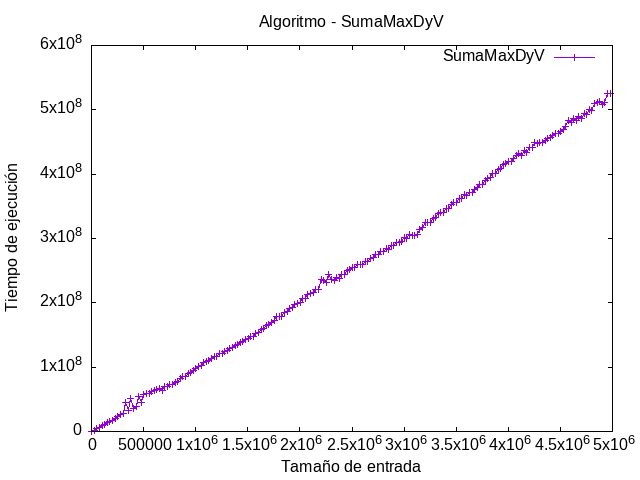
\includegraphics[width=0.7\linewidth]{assets/Img/SumaMaxDyV.png}
            \caption{Ejecución algoritmo SumaMaxDyV}
            \label{fig:SumaMaxDyV}
      \end{figure}
\end{center}
\newpage
\subsection{Estudio híbrido}
\begin{center}
      \begin{figure}[h]
            \centering
            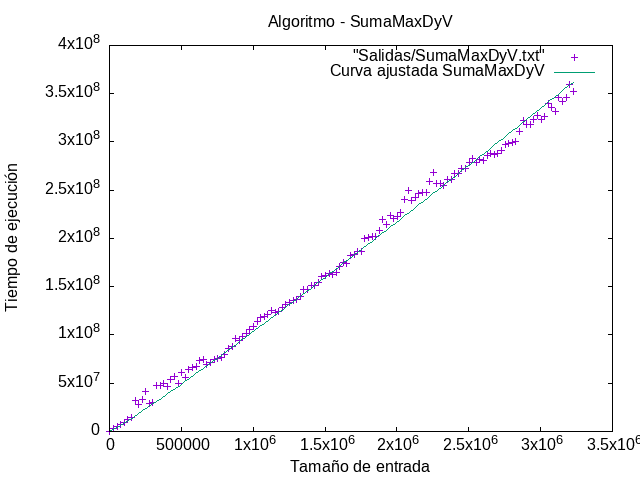
\includegraphics[width=0.7\linewidth]{assets/Img/SumaMaxDyV_hib.png}
            \caption{Ajuste híbrido algoritmo SumaMaxDyV}
            \label{fig:sumaMax}
      \end{figure}
\end{center}
Tras la interpretación de los datos empíricos en gnuplot y de la formula teorica del métoco, obtenemos que \\
las constantes ocultas son:
\begin{equation*}
      T_{SumaMaxDyV}=1.65508x + 0.991967
\end{equation*}

\section{Problema 2: Enlosar un espacio }


\section{Problema 3: Problema del viajante de comercio.}
Para el tercer problema, nos encontramos ante un problema de complejidad
NP-duro, por lo que no podemos encontrar una solución exacta en tiempo polinómico.
Sin embargo, podemos encontrar una solución aproximada aplicando la técnica de Divide y Vencerás.
Para ello, usamos el algoritmo de fuerza bruta para encontrar la solución exacta para subconjuntos
del problema total y luego unimos las soluciones parciales para obtener una solución que se optimiza
para asegurar un cierto mínimo de precision.

\subsection{Estudio Empírico}
Para determinar el umbral con el que obtenemos la mejor relación entre eficiencia y precisión, hemos
realizado una serie de pruebas con diferentes valores de umbral, a partir de tamaño 10, el algoritmo de
fuerza bruta se vuelve completamente inviable, de forma similar, para tamaño menor a 4, el algoritmo
no nos produce ninguna mejora en cuanto a eficiencia debido a la cantidad de llamadas recursivas que
saturan la pila, y la precision disminuye de forma considerable. Por ello, hemos decidido realizar
las pruebas para tamaños de 4 a 10, con distintas ciudades con solución ya conocida, para comparar
los tiempos de ejecución y la precisión de los resultados obtenidos:
\subsubsection*{Tiempo de ejecución}
\begin{center}
      \begin{figure}[H]
            \centering
            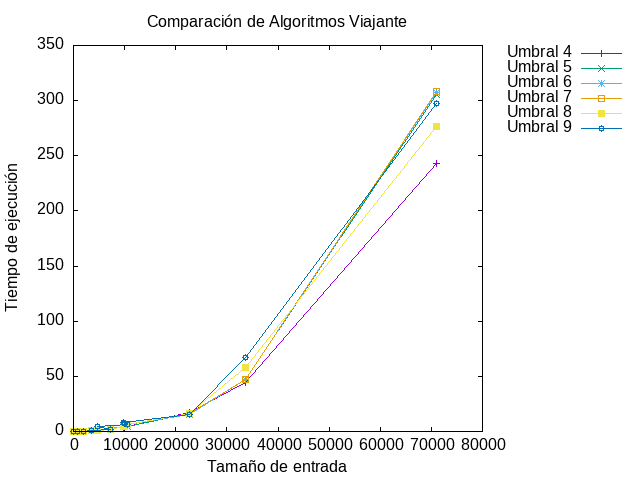
\includegraphics[width=0.7\linewidth]{assets/Img/UmbralP3.png}
            \caption{Ejecución algoritmo Viajante}
            \label{fig:Viajante}
      \end{figure}
\end{center}
Como se puede apreciar, los mejores resultados se han obtenido con los umbrales {4,8}.
Para decididir cual de los dos umbrales es el mejor, nos fijamos en la precisión
que nos proporciona cada uno de ellos:
\subsubsection*{Precisión}



\chapter{Conclusiones}
\end{document}